\documentclass{article}
\usepackage[utf8]{inputenc}
\usepackage{graphicx}
\usepackage{hyperref}
\usepackage{biblatex}

\bibliography{main.bib}

\title{Vault: An End-to-End Encrypted File Sharing Service}
\author{Justin Stanley}
\date{May 11, 2022}

\begin{document}

\maketitle

\section{Problem}
Since their inception, file hosting services have become extremely popular among Internet users. People use these services to store important documents, pictures, and other files. These files often need to be shared with other users on the platform. In the modern age of cloud computing, due to data and computation outsourcing much of this data is stored and manipulated on potentially untrustworthy infrastructure. To protect user privacy, sensitive data must be encrypted when it is stored. However, if the encryption keys are stored on the server, a malicious actor can retrieve the keys from the server to decrypt user files. My project moves file encryption to the client side, so all user data is encrypted before it is ever sent to the server. Furthermore, the authentication process also secures the user's password, so a malicious server cannot steal the user's credentials for use on other services. I implemented a file sharing feature, so users can share files with other users on the platform securely, using fingerprint identification to ensure the server cannot intercept shared file data. The project is built from scratch with no reused existing code. I have deployed the project to AWS under an auto-scaling group, so it can scale to a large number of users.

\section{Design}
The system consists of 3 primary components: \textbf{backend}, \textbf{frontend} and \textbf{storage}.
\subsection{Backend}
The backend exposes a REST API by which the frontend can interact with the system. The backend also serves the frontend HTML through this API. This component runs on AWS EC2 instances and has access to the S3 secret keys, which it uses directly to upload and download files from S3.
\subsection{Frontend}
The frontend is an HTML page which users interact with to use the service. A login prompt is initially displayed which the users can login and register with. After a valid authentication token is obtained, the users are directed to a list of their available files. Users can see files which they have uploaded as well as files which have been shared with them. Users can share and download each file available in the list. Finally, users can see their current username and key fingerprint at the bottom of the screen.
\subsection{Storage}
The service uses S3 to store all user data. At the top level of the bucket is a folder named \texttt{users}, which contains a folder for each user designated by their username. Each user folder contains a directory \texttt{files} which contains each file owned by or shared to the user. Every user folder contains a file \texttt{token} which contains the user's current authorization token and expiration date. Finally, each user folder has a file \texttt{info} which contains the user's username, public key and encrypted private key.
\section{Implementation}
\subsection{Backend}
The backend is written using Node.js as an asynchronous web application. Express.js\cite{exp} is used to serve web requests, and the AWS API is used to make requests to S3. All requests are handled asynchronously using async/await or callback methods.

The REST API is defined as follows:

\noindent
\begin{figure}
    \centering
\begin{tabular}{l | l}
    \texttt{GET /} & Serves the front-end HTML. \\ \\
    \texttt{POST /api/register} & Creates a user account. Expects parameters: \\
    & \texttt{username}, \texttt{privateKey}, \texttt{publicKey} \\ \\
    \texttt{POST /api/preauth} & Starts an auth handshake. Expects parameters: \\
    & \texttt{username} \\
    & Server responds with \texttt{encPrivateKey}, \texttt{encNonce} \\ \\
    \texttt{POST /api/auth} & Finishes an auth handshake. Expects parameters: \\
    & \texttt{username}, \texttt{nonce} \\
    & Server responds with \texttt{username}, \texttt{token}, \texttt{expiration} \\ \\
    \small{\texttt{POST /api/download/<user>/<path>}} & Downloads a user file. Expects \texttt{token} in request body. \\
    & Server responds with \texttt{\{ keys, filedata \}} \\ \\
    \small{\texttt{PUT /api/upload/<user>/<path>}} & Uploads a user file. Expects \texttt{token} in request body. \\ \\
    \texttt{POST /api/key/<user>} & Retrieves a user's public key. \\
    & Server responds with \texttt{\{ publicKey \}} \\  \\
    \texttt{POST /api/tree/<user>} & Retrieves a list of a user's files. Expects \texttt{token} in body. \\
    & Server responds with \texttt{\{ publicKey \}} \\  \\
\end{tabular}
    \caption{Backend REST API}
    \label{fig:rest}
\end{figure}

\subsection{Frontend}
The frontend is written in Pug which is then compiled to HTML by the backend. The WebCrypto API\cite{w3c} is used to perform client-side encryption. RSA-OAEP\cite{rsa} is used for asymmetric encryption, while AES-256\cite{aes} is used for symmetric encryption. I heavily referenced the public Mozilla WebCrypto API manual\cite{moz} while developing the frontend. The major methods are described below.

\subsubsection{Register}
To register, a user generates a keypair. A random 16-byte \texttt{salt} is generated. The user's password is used along with PBKDF2 to generate a 16-byte \texttt{key}. A random 16-byte \texttt{iv} is generated. The \texttt{iv} and \texttt{key} are then used to encrypt the private key with AES-256-CBC\cite{aes}. The username, public key, encrypted private key, and \texttt{salt}, \texttt{iv} are sent to the backend. The server responds with success or failure.

\subsubsection{Login}
To login, a client first sends a pre-auth request to the server with their username. The server responds with an encrypted private key, \texttt{salt}, \texttt{iv}, and an encrypted nonce. The client uses the \texttt{salt} and password to generate a \texttt{key} as done during register. The \texttt{key} is used to decrypt the private key, which is then used to decrypt the nonce. The decrypted nonce is sent back to the server (as proof of ownership of the private key). The server then responds with an authentication token.

\subsubsection{Upload}
To upload a file, the user generates a random \texttt{iv}, \texttt{key} and uses them to encrypt the file. The \texttt{key} and \texttt{iv} are then encrypted with the user's own public key and bundled with the file. The bundle is sent to the server along with an auth token, username and upload path.

\subsubsection{Download}
To download a file the user simply sends their token along with the desired file path to the server. The server verifies the token is valid and sends the file data. The frontend then retrieves the \texttt{key} and \texttt{iv} by decrypting the file data header with the user's private key. The keys are then used to decrypt the file, and the user is prompted to save the decrypted file.

\subsubsection{Share}
To share a file, the user firsts downloads the file into local memory as in \emph{download}. The user then sends a \texttt{get-key} request to retrieve the destination user's public key. The user is shown the destination public key fingerprint to verify it is correct. After confirming, the user re-encrypts the file data as in \emph{upload}, but with the other user's public key. A \texttt{share} request is then sent to the server which allows the user to upload files to another's storage. The new file is saved as \texttt{shared/<origin\_user>/<path>} to avoid overwriting existing files.

\section{User guide}

\subsection{Installation/Requirements}
To install and use the application, first ensure your machine has the appropriate AWS configuration so the backend can access S3. On Linux, this file should be located at \texttt{\$HOME/.aws/credentials}. You must have OpenSSL along with its command line utilities installed. In your S3 dashboard, create a new bucket named \texttt{coms559-project-vault}. Proceed to install Node.js by following the instructions for your operating system at \url{https://nodejs.org}. Clone the project repository from \url{https://github.com/codeandkey/coms559-project-vault/} if you do not already have it.

Run the following commands within the repository folder to download dependencies and initialize SSL keys:

\begin{figure}
    \centering
    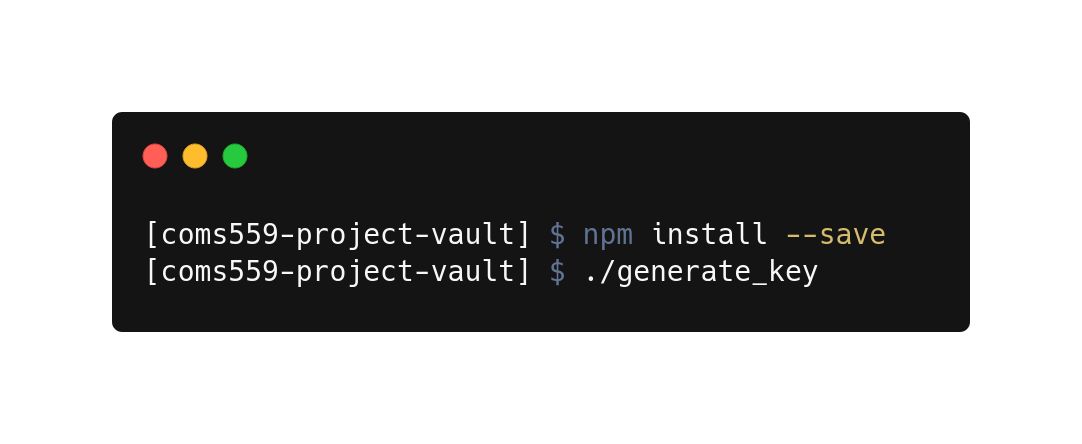
\includegraphics[scale=0.35]{carbon(3).png}
    \caption{Installation commands}
    \label{fig:commands}
\end{figure}

\subsection{Starting}
After installation is finished, start the backend with the command:

\texttt{\$ node backend.js}.

\subsection{Usage}
Once the backend is running, open a web browser supporting the WebCrypto standard (most modern browsers will) and navigate to \url{http://localhost:8080/}. A prompt will appear allowing you to enter a username and password to register as shown in figure \ref{fig:login}. After registering you will be brought to a page with your files and utilities as shown in figure \ref{fig:frontpage}. At the bottom of the page you will see your username along with your key fingerprint. You are encouraged to share this fingerprint in advance with users you may share files with. On the left is an ``Upload" button which you can click to upload a new file. Once you have uploaded a file you will see the ``Download" and ``Share" buttons next to the listed file, which you can click to download and share the file with other users respectively. When sharing a file with another user, you will be prompted for their username and then shown their fingerprint. Once you have verified their fingerprint is correct the file will be shared with them.

\begin{figure}
    \centering
    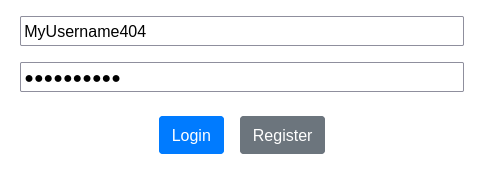
\includegraphics[scale=0.7]{login.png}
    \caption{Login page}
    \label{fig:login}
\end{figure}

\begin{figure}
    \centering
    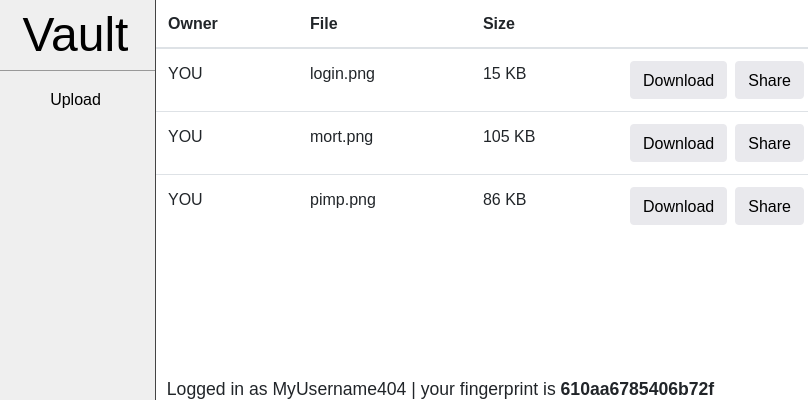
\includegraphics[scale=0.5]{frontpage_000.png}
    \caption{Main activity page}
    \label{fig:frontpage}
\end{figure}

\section{Self-evaluation}

I feel most of the major goals of this project were accomplished. All encryption is performed client-side and user files as well as user credentials are protected without any need for server security. However, there are multiple drawbacks to the system as it is:

\begin{itemize}
    \item The system does not support data streaming. As WebCrypto does not support streaming cryptography, the entire file data must be stored in the browser memory before encrypting or decrypting. Storing large files in RAM is often not acceptable for large files (\texttt{> 8GB}). To fix this, it may be necessary to break the file into blocks on the client side, and then encrypt them one at a time before sending them to the server.
    \item Currently users must share their public key fingerprints to each other outside of the system to guarantee security. I do not see any way around this, and it may be highly inconvienent for users to store each others fingerprints. \item Fingerprints are currently based on the first 8 bytes of the SHA-512 hash of the SPKI-encoded public key. This may not be sufficient- it may be possible for an adversary to easily generate a key with the same fingerprint in a reasonable amount of time, allowing them to impersonate another user.
\end{itemize}

\printbibliography



\end{document}

